\pdfoutput=1
% In particular, the hyperref package requires pdfLaTeX in order to break URLs across lines.

\documentclass[11pt]{article}

% Change "review" to "final" to generate the final (sometimes called camera-ready) version.
% Change to "preprint" to generate a non-anonymous version with page numbers.
\usepackage[preprint]{acl}

% Standard package includes
\usepackage{times}
\usepackage{latexsym}

% For proper rendering and hyphenation of words containing Latin characters (including in bib files)
\usepackage[T1]{fontenc}
% For Vietnamese characters
% \usepackage[T5]{fontenc}
% See https://www.latex-project.org/help/documentation/encguide.pdf for other character sets

% This assumes your files are encoded as UTF8
\usepackage[utf8]{inputenc}

% This is not strictly necessary, and may be commented out,
% but it will improve the layout of the manuscript,
% and will typically save some space.
\usepackage{microtype}

% This is also not strictly necessary, and may be commented out.
% However, it will improve the aesthetics of text in
% the typewriter font.
\usepackage{inconsolata}

%Including images in your LaTeX document requires adding
%additional package(s)
\usepackage{graphicx}
\usepackage{hyperref}

% If the title and author information does not fit in the area allocated, uncomment the following
%
%\setlength\titlebox{<dim>}
%
% and set <dim> to something 5cm or larger.

\title{Etude comparative de vecteurs pour l'identification du parti politique d'interventions parlementaires}

% Author information can be set in various styles:
% For several authors from the same institution:
\author{Pauline Degez \and Florian Philippe \and Valentine Fleith \\
         Address line \\ ... \\ 43017467@parisnanterre.fr}
% if the names do not fit well on one line use
%         Author 1 \\ {\bf Author 2} \\ ... \\ {\bf Author n} \\
% For authors from different institutions:
% \author{Author 1 \\ Address line \\  ... \\ Address line
%         \And  ... \And
%         Author n \\ Address line \\ ... \\ Address line}
% To start a separate ``row'' of authors use \AND, as in
% \author{Author 1 \\ Address line \\  ... \\ Address line
%         \AND
%         Author 2 \\ Address line \\ ... \\ Address line \And
%         Author 3 \\ Address line \\ ... \\ Address line}

%\author{First Author \\
  %Affiliation / Address line 1 \\
  %Affiliation / Address line 2 \\
  %Affiliation / Address line 3 \\
  %\texttt{email@domain} \\\And
  %Second Author \\
  %Affiliation / Address line 1 \\
  %Affiliation / Address line 2 \\
  %Affiliation / Address line 3 \\
  %\texttt{email@domain} \\}

%\author{
%  \textbf{First Author\textsuperscript{1}},
%  \textbf{Second Author\textsuperscript{1,2}},
%  \textbf{Third T. Author\textsuperscript{1}},
%  \textbf{Fourth Author\textsuperscript{1}},
%\\
%  \textbf{Fifth Author\textsuperscript{1,2}},
%  \textbf{Sixth Author\textsuperscript{1}},
%  \textbf{Seventh Author\textsuperscript{1}},
%  \textbf{Eighth Author \textsuperscript{1,2,3,4}},
%\\
%  \textbf{Ninth Author\textsuperscript{1}},
%  \textbf{Tenth Author\textsuperscript{1}},
%  \textbf{Eleventh E. Author\textsuperscript{1,2,3,4,5}},
%  \textbf{Twelfth Author\textsuperscript{1}},
%\\
%  \textbf{Thirteenth Author\textsuperscript{3}},
%  \textbf{Fourteenth F. Author\textsuperscript{2,4}},
%  \textbf{Fifteenth Author\textsuperscript{1}},
%  \textbf{Sixteenth Author\textsuperscript{1}},
%\\
%  \textbf{Seventeenth S. Author\textsuperscript{4,5}},
%  \textbf{Eighteenth Author\textsuperscript{3,4}},
%  \textbf{Nineteenth N. Author\textsuperscript{2,5}},
%  \textbf{Twentieth Author\textsuperscript{1}}
%\\
%\\
%  \textsuperscript{1}Affiliation 1,
%  \textsuperscript{2}Affiliation 2,
%  \textsuperscript{3}Affiliation 3,
%  \textsuperscript{4}Affiliation 4,
%  \textsuperscript{5}Affiliation 5
%\\
%  \small{
%    \textbf{Correspondence:} \href{mailto:email@domain}{email@domain}
%  }
%}

\begin{document}
\maketitle
\begin{abstract}
This document is a supplement to the general instructions for *ACL authors. It contains instructions for using the \LaTeX{} style files for ACL conferences.
The document itself conforms to its own specifications, and is therefore an example of what your manuscript should look like.
These instructions should be used both for papers submitted for review and for final versions of accepted papers.
\end{abstract}

% \section{Introduction}
\section{Introduction}

\par La cinquième édition du défi Fouille de Textes (DEFT) porte sur la fouille d'opinions sur des corpus multilingues. Trois tâches ont été proposées,
dans trois langues : le français, l'anglais et l'italien. Cet article se concentre sur la 3ème tâche, dont l'objet est l'identification automatique
du parti politique d'appartenance de chacun des intervenants dans un corpus de débats parlementaires européens. Il s'agit d'une tâche de classification à 5 classes:
\texttt{Verts-ALE}, \texttt{GUE-NGL}, \texttt{PSE}, \texttt{ELDR} et \texttt{PPE-DE}.

\par Le but de nos expériences sera ainsi de trouver un/des classifieur(s) permettant de réaliser cette tâche. Pour ce faire, nous utiliserons les algorithmes
de Machine Learning implementés dans la bibliothèque Python \texttt{scikit-learn}.

\subsection{Travaux présentés en 2009}




\begin{table}[h!]
\centering
\setlength{\tabcolsep}{5pt} % Réduit l'espace entre les colonnes
\renewcommand{\arraystretch}{1.2} % Ajuste la hauteur des lignes
\resizebox{\columnwidth}{!}{ % Ajuste la largeur à une demi-colonne
\begin{tabular}{@{}c| c| c| c| c| c@{}}
\textbf{Parti} & \textbf{ELDR} & \textbf{GUE-NGL} & \textbf{PPE-DE} & \textbf{PSE} & \textbf{Verts/ALE} \\
\hline
F-mesure & 0.21 & 0.37 & 0.47 & 0.37 & 0.25 \\ 
\end{tabular}
}
\caption{Moyennes des F-mesures par parti politique.}
\label{tab:moyennes_fmesures}
\end{table}


\par En 2009, un seul participant a soumis un travail pour la tâche 3 ; la Présentation de l'édition 2009 \hyperlink{ref1}{[1]}\footnote{Actes du cinquième défi fouille de texte, DEFT2009, Paris, France, 22 juin 2009} évoque, pour expliquer cela, les faibles résultats des logiciels sur cette tâche, bien que conformes à ceux que des humains obtiendraient manuellement. L'équipe de l'Université de Montréal (D. Forest and al.) a obtenu en moyenne les f-mesures présentées dans la \hyperref[tab:moyennes_fmesures]{Table 1}. En moyenne, cela donne donc une f-mesure 0.331.

\subsection{Notre approche et travaux antérieurs}

Pour ce travail, notre approche a été comparative sur plusieurs niveaux. Tout d'abord, nous comparons différents classifieurs : \texttt{Random Forest}, \texttt{Régression logistique}, \texttt{Perceptron} et \texttt{Support Vector Machine}. De plus, nous testons aussi différentes vectorisations du corpus sur l'ensemble de ces modèles: \texttt{TF-IDF}, \texttt{Doc2Vec}, et des \texttt{Bert embeddings}.


\par Plusieurs travaux de recherches explorent les comparaisons entre performances des modèles selon les techniques de vectorisation utilisées. Nous pouvons par exemples évoquer ceux de P. Joseph et S. Y. Yerima~\hyperlink{ref1}{[1]} \footnote{P. Joseph and S. Y. Yerima, "A comparative study of word embedding techniques for SMS spam detection," 2022 14th International Conference on Computational Intelligence and Communication Networks (CICN), Al-Khobar, Saudi Arabia, 2022, pp. 149-155,} en 2022, qui compare les performances des N-grams, TF-IDF, Sac de mots, Word2Vec, Doc2Vec, etc. Leur objectif est de comparer l'impact de la vectorisation sur la précision des modèles. Dans leur article, les modèles \texttt{Doc2Vec} et \texttt{TF-IDF} démontrent de bons résultats, nous allons ainsi les tester dans notre expérience. Nous décidons d'ajouter à ces deux dernier les embeddings de \texttt{BERT} afin d'avoir trois techniques variées : une méthode statistique, une méthode fondée sur un ANN classique et une sur un Transformer.




% \section{Engines}
\section{Méthode}

\subsection{Dataset}

Nous utilisons le dataset fournit pour la tâche 3 de l’édition 2009 de DEFT.
Il s'agit d'un corpus multilingue de débats parlementaires européens. Chaque intervention
parlementaire est classée en fonction du parti \footnote {ELDR, PPE-DE, PSE, GUE-NGL et Verts-ALE}
du locuteur et présente dans le corpus dans 3 langues : anglais, français et italien.\\
Au moment de faire des statistiques descriptives, nous nous sommes rendus comptes 
que le corpus présentait des doublons, et ce majoritairement dans la partition test.
\begin{figure}[ht]
    \centering
    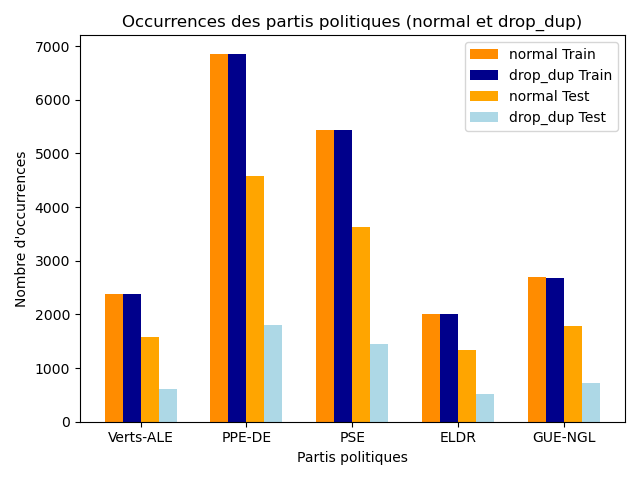
\includegraphics[width=\columnwidth]{../stats/occurences_orig_vs_drop_dup_par_cat.png}
    \caption{Nombre d'interventions par parti par partition test/train, dans le corpus original et dans la version sans doublons}
    \label{fig:barplot_dataset}
\end{figure}

Après suppression des doublons, la partition prévu (40/60) est changée : elle est 
maintenant de 20/80\footnote{ 0.79 pour le train et 0.21 pour le test}.
Nous avons envisagé de refaire le partitionnement pour réimplémenter le partitionnement 
prévu, mais avons renoncé pour deux raisons : 
refaire le partitionnement nous éloigne, encore, du corpus initialement prévu, et les 
résultats de quelques modèles sur un corpus repartitionné étaient proches des résultats 
sur cette partition 80/20.
Par ailleurs, la répartition des classes est déséquilibrée : les classes PPE-DE et PSE forment à elles deux 63,5 \% du corpus. Ceci devra être 
pris en compte dans le prétraitement.\footnote{la figure correspond au train, mais la répartition est sensiblement la même dans le test}

\begin{table}[ht]
    \centering
\begin{tabular}{|l|l|l|}
\hline
Statistique & Test & train 3 \\ \hline
Moyenne & 3871.4 & 1021.2 \\ \hline
STD & 2149.1 & 569.7 \\ \hline
Min & 2005.0 & 525.0 \\ \hline
1er quartile & 2376.0 & 615.0 \\ \hline
Médiane & 2687.0 & 715.0\\ \hline
3eme quartile & 5431.0 & 1448.0\\ \hline
Max & 6858.0 & 1803.0\\ \hline
\end{tabular}
\caption{Nombres d'intervention par parti par partition}
\label{tab:stats_dataset}
\end{table}

\begin{figure}[ht]
    \centering
    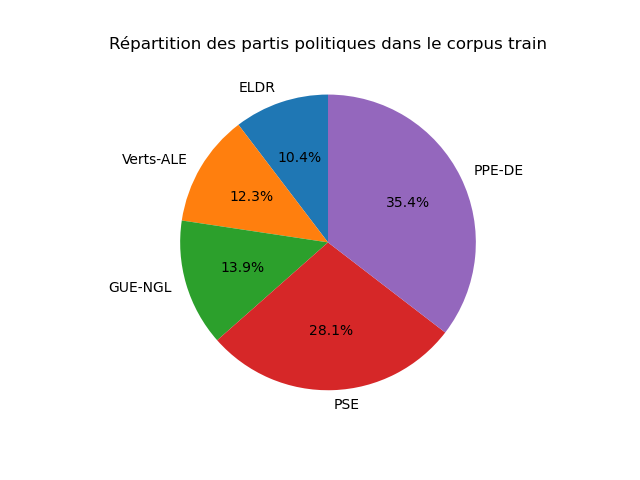
\includegraphics[width=\columnwidth]{../stats/occurences_par_partis_train_camember.png}
    \caption{Répartition des interventions par parti dans la partition train sans doublons}
    \label{fig:camember_dataset}
\end{figure}
\subsection{Prétraitements}
Le texte des interventions a été soumis à un prétraitement simple :\\
\indent(1) Suppresion de la ponctuation\\
\indent(2) Unification de la casse en minuscules\\
\indent(3) Tokenisation\footnote {Une lemmatisation avec la bibliothèque SpaCy a été envisagée,
mais ce corpus multilingue aurait nécessité le chargement de 3 modèles linguistiques
différents et ralongé d'autant le temps de traitement}
\\
Pour résoudre le problème de déséquilibre des classes, nous avons opté pour le \textit{downsampling} afin d'obtenir des classes relativement équilibrées,
en utilisant la fonction \textit{resample} de la bibliothèque Sckit-learn.

\begin{table}[ht]
    \centering
\begin{tabular}{|l|l|l|}
\hline
Parti & Test & train 3 \\ \hline
Moyenne & 3871.4 & 1021.2 \\ \hline
STD & 2149.1 & 569.7 \\ \hline
Min & 2005.0 & 525.0 \\ \hline
1er quartile & 2376.0 & 615.0 \\ \hline
Médiane & 2687.0 & 715.0\\ \hline
3eme quartile & 5431.0 & 1448.0\\ \hline
Max & 6858.0 & 1803.0\\ \hline
\end{tabular}
\caption{Nombres d'intervention par parti par partition}
\label{tab:stats_dataset}
\end{table}


\subsection{Les différents embeddings}

\section{Résultats}

Comme mentionné en introduction, nous avons testé trois méthodes de vectorisation : TF-IDF, doc2vec et BERT
Nous avons utilisé ces vecteurs pour entraîner et comparer 4 modèles différents : Régression logistique, SVM, Random Forest et Perceptron.

\subsection{Vecteurs TF-IDF}

\begin{figure}[t]
  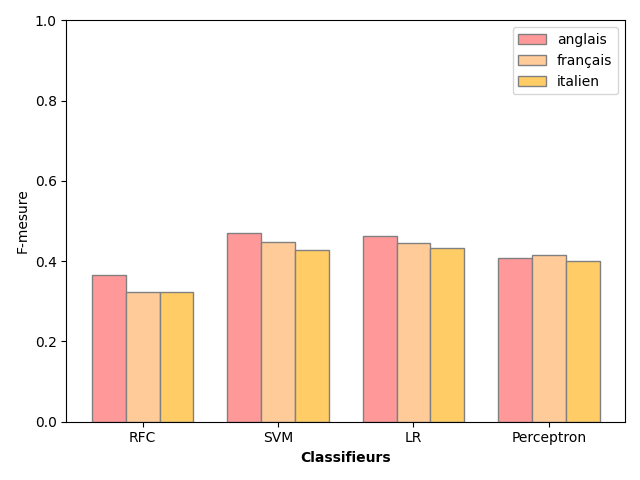
\includegraphics[width=\columnwidth]{assets/comparaison_metriques_tfidf.png}
  \caption{A figure with a caption that runs for more than one line.
    Example image is usually available through the \texttt{mwe} package
    without even mentioning it in the preamble.}
  \label{fig:tfidf_comparison}
\end{figure}

Les meilleurs résultats que nous ayons obtenus sont ceux avec un vectorisation tf-idf.
On peut voir sur la figure~\ref{fig:tfidf_comparison} que nous avons obtenu au mieux : 0.46 en anglais avec un SVM, 0.43 en italien avec une régression linéaire et 0.44 en français avec un SVM.

\section{Preamble}

The first line of the file must be
\begin{quote}
\begin{verbatim}
\documentclass[11pt]{article}
\end{verbatim}
\end{quote}

To load the style file in the review version:
\begin{quote}
\begin{verbatim}
\usepackage[review]{acl}
\end{verbatim}
\end{quote}
For the final version, omit the \verb|review| option:
\begin{quote}
\begin{verbatim}
\usepackage{acl}
\end{verbatim}
\end{quote}

To use Times Roman, put the following in the preamble:
\begin{quote}
\begin{verbatim}
\usepackage{times}
\end{verbatim}
\end{quote}

Please see the \LaTeX{} source of this document for comments on other packages that may be useful.


By default, the box containing the title and author names is set to the minimum of 5 cm. If you need more space, include the following in the preamble:
\begin{quote}
\begin{verbatim}
\setlength\titlebox{<dim>}
\end{verbatim}
\end{quote}
where \verb|<dim>| is replaced with a length. Do not set this length smaller than 5 cm.

\section{Document Body}

\subsection{Footnotes}


\subsection{Tables and figures}

See Table~\ref{tab:accents} for an example of a table and its caption.
\textbf{Do not override the default caption sizes.}

\begin{table}
  \centering
  \begin{tabular}{lc}
    \hline
    \textbf{Command} & \textbf{Output} \\
    \hline
    \verb|{\"a}|     & {\"a}           \\
    \verb|{\^e}|     & {\^e}           \\
    \verb|{\`i}|     & {\`i}           \\
    \verb|{\.I}|     & {\.I}           \\
    \verb|{\o}|      & {\o}            \\
    \verb|{\'u}|     & {\'u}           \\
    \verb|{\aa}|     & {\aa}           \\\hline
  \end{tabular}
  \begin{tabular}{lc}
    \hline
    \textbf{Command} & \textbf{Output} \\
    \hline
    \verb|{\c c}|    & {\c c}          \\
    \verb|{\u g}|    & {\u g}          \\
    \verb|{\l}|      & {\l}            \\
    \verb|{\~n}|     & {\~n}           \\
    \verb|{\H o}|    & {\H o}          \\
    \verb|{\v r}|    & {\v r}          \\
    \verb|{\ss}|     & {\ss}           \\
    \hline
  \end{tabular}
  \caption{Example commands for accented characters, to be used in, \emph{e.g.}, Bib\TeX{} entries.}
  \label{tab:accents}
\end{table}

As much as possible, fonts in figures should conform
to the document fonts. See Figure~\ref{fig:experiments} for an example of a figure and its caption.

environment at an appropriate point within the text.
The \verb|graphicx| package supports various optional arguments to control the
appearance of the figure.
You must include it explicitly in the \LaTeX{} preamble (after the
\verb|\documentclass| declaration and before \verb|\begin{document}|) using
\verb|\usepackage{graphicx}|.

\begin{figure}[t]
  \includegraphics[width=\columnwidth]{example-image-golden}
  \caption{A figure with a caption that runs for more than one line.
    Example image is usually available through the \texttt{mwe} package
    without even mentioning it in the preamble.}
  \label{fig:experiments}
\end{figure}

\begin{figure*}[t]
  \includegraphics[width=0.48\linewidth]{example-image-a} \hfill
  \includegraphics[width=0.48\linewidth]{example-image-b}
  \caption {A minimal working example to demonstrate how to place
    two images side-by-side.}
\end{figure*}

\subsection{Hyperlinks}

Users of older versions of \LaTeX{} may encounter the following error during compilation:
\begin{quote}
\end{quote}
This happens when pdf\LaTeX{} is used and a citation splits across a page boundary. The best way to fix this is to upgrade \LaTeX{} to 2018-12-01 or later.

\subsection{Citations}


Table~\ref{citation-guide} shows the syntax supported by the style files.
We encourage you to use the natbib styles.
You can use the command \verb|\citet| (cite in text) to get ``author (year)'' citations, like this citation to a paper by \citet{Gusfield:97}.
You can use the command \verb|\citep| (cite in parentheses) to get ``(author, year)'' citations \citep{Gusfield:97}.
You can use the command \verb|\citealp| (alternative cite without parentheses) to get ``author, year'' citations, which is useful for using citations within parentheses (e.g. \citealp{Gusfield:97}).

A possessive citation can be made with the command \verb|\citeposs|.
This is not a standard natbib command, so it is generally not compatible
with other style files.

\subsection{References}

\nocite{Ando2005,andrew2007scalable,rasooli-tetrault-2015,Gusfield:97}

The \LaTeX{} and Bib\TeX{} style files provided roughly follow the American Psychological Association format.
If your own bib file is named \texttt{custom.bib}, then placing the following before any appendices in your \LaTeX{} file will generate the references section for you:
\begin{quote}
\begin{verbatim}
\bibliography{custom}
\end{verbatim}
\end{quote}

You can obtain the complete ACL Anthology as a Bib\TeX{} file from \url{https://aclweb.org/anthology/anthology.bib.gz}.
To include both the Anthology and your own .bib file, use the following instead of the above.
\begin{quote}
\begin{verbatim}
\bibliography{anthology,custom}
\end{verbatim}
\end{quote}

Please see Section~\ref{sec:bibtex} for information on preparing Bib\TeX{} files.

\subsection{Equations}

An example equation is shown below:
\begin{equation}
  \label{eq:example}
  A = \pi r^2
\end{equation}

Labels for equation numbers, sections, subsections, figures and tables
are all defined with the \verb|\label{label}| command and cross references
to them are made with the \verb|\ref{label}| command.

This an example cross-reference to Equation~\ref{eq:example}.

\bibliography{custom}

\subsection{Appendices}

Use \verb|\appendix| before any appendix section to switch the section numbering over to letters. See Appendix~\ref{sec:appendix} for an example.

\section{Bib\TeX{} Files}
\label{sec:bibtex}

Unicode cannot be used in Bib\TeX{} entries, and some ways of typing special characters can disrupt Bib\TeX's alphabetization. The recommended way of typing special characters is shown in Table~\ref{tab:accents}.

Please ensure that Bib\TeX{} records contain DOIs or URLs when possible, and for all the ACL materials that you reference.
Use the \verb|doi| field for DOIs and the \verb|url| field for URLs.
If a Bib\TeX{} entry has a URL or DOI field, the paper title in the references section will appear as a hyperlink to the paper, using the hyperref \LaTeX{} package.

\section*{Acknowledgments}

This document has been adapted
by Steven Bethard, Ryan Cotterell and Rui Yan
from the instructions for earlier ACL and NAACL proceedings, including those for
ACL 2019 by Douwe Kiela and Ivan Vuli\'{c},
NAACL 2019 by Stephanie Lukin and Alla Roskovskaya,
ACL 2018 by Shay Cohen, Kevin Gimpel, and Wei Lu,
NAACL 2018 by Margaret Mitchell and Stephanie Lukin,
Bib\TeX{} suggestions for (NA)ACL 2017/2018 from Jason Eisner,
ACL 2017 by Dan Gildea and Min-Yen Kan,
NAACL 2017 by Margaret Mitchell,
ACL 2012 by Maggie Li and Michael White,
ACL 2010 by Jing-Shin Chang and Philipp Koehn,
ACL 2008 by Johanna D. Moore, Simone Teufel, James Allan, and Sadaoki Furui,
ACL 2005 by Hwee Tou Ng and Kemal Oflazer,
ACL 2002 by Eugene Charniak and Dekang Lin,
and earlier ACL and EACL formats written by several people, including
John Chen, Henry S. Thompson and Donald Walker.
Additional elements were taken from the formatting instructions of the \emph{International Joint Conference on Artificial Intelligence} and the \emph{Conference on Computer Vision and Pattern Recognition}.

% Bibliography entries for the entire Anthology, followed by custom entries
%\bibliography{anthology,custom}
% Custom bibliography entries only
\bibliography{custom}

\appendix

\section{Example Appendix}
\label{sec:appendix}

This is an appendix.

\end{document}
